\documentclass[../main.tex]{subfiles}
\graphicspath{{\subfix{../figures/}}}

\begin{document}
\chapter{tidyqpcr: Quantitative PCR Analysis in the tidyverse}

\section{Chapter 3 Introduction}

Quantitative PCR is the most common technique for the quantification of DNA and RNA. 
The specificity and sensitively of the assay, as described above, has led it to be considered the gold standard for nucleotide detection and quantification in medicine, legislation and academia \parencite{Kubista2006}.
However, qPCR experiments, especially assays requiring a reverse transcriptase step, are susceptible to several reliability issues if poorly designed \parencite{Bustin2002}.
Nevertheless, the widespread use of qPCR across distinct disciplines has enabled the creation of countless protocols, equipment and analysis methods without consistent standards \parencite{Bustin2021}.
The limitations and varying quality of qPCR experiments has lead to a reproducibility crisis with significant consequences for academic rigour \parencite{Garson2009} and public health \parencite{Bustin2013}. 

qPCR assays are susceptible to multiple biases that can cause highly variable or unrepeatable results \parencite{Bustin2002}.
Lab specific protocols for extraction, pipetting and storage can introduce variation, with samples having $R^2 = 0.4$ between extraction methods \parencite{Bustin2017, Dagnall2017}.
A sample's position on a qPCR plate can also have a significant contribution to measured expression with one study showing $10\%$ of the variation between replicates was due to well position \parencite{Eisenberg2015}. 
Positional effects can be introduced as edge wells may be more susceptible to evaporation or thermal gradients may be uneven across the plate. 
Finally, the reverse transcription step in qPCR experiments using cDNA, such as mRNA quantification, can cause 91-fold changes in Cq values \parencite{Stahlberg2004}. 
The choice of reverse transcriptase and sensitivity to original RNA concentration have been documented sources of variation since the introduction of a reverse transcription step.
The effect is target specific as different reverse transcriptases interactive with RNA secondary structures in different ways \parencite{Brooks1995, Williams1992}.

In an effort to improve the reproducibility of qPCR results a team of qPCR experts created guidelines for publishing qPCR results called the Minimum Information for the Publication of Quantitative Real-Time PCR Experiments (MIQE) guidelines \parencite{Bustin2009}.
They provide a thorough checklist of every detail that needs to be reported in order to enable another researcher to accurately repeat your work. 
Over time they developed their own file format, the Real-Time PCR Data Markup Language or RDML, to standardise the way scientists describe their experiments which users can upload to a bespoke open source database \parencite{Lefever2009, Ruijter2015}.
The guidelines have been around for over a decade, but they are still not widely implemented with as little as $4\%$ of qPCR articles citing them \parencite{AbdelNour2020}.

In order to improve the reproducibility of qPCR analyses and promote the usage of MIQE guidelines, we propose the the development of a novel analysis package that uses detailed documentation and open software practices to teach and facilitate transparent, open access and quality controlled qPCR analysis. 
In addition, the dependence on proprietary qPCR machine software for the calculation of threshold Cq values and quality control graphs remains a stumbling block for reproducible and trustworthy analysis. 
We believe a novel package developed in the programming language R, a common language used in biology, could increase the quality of qPCR assays from initial experimental design to final publication of results.
The consistent structure of qPCR data also provides an opportunity to apply the latest data analysis practices.
Threshold Cq values are the raw output of any qPCR machine which are inherently separated into values from independent wells. 
Therefore, developing functions that can take advantage of this regular, independent structure to Cq values can lead to comprehensive and efficient analysis of data sets of varying sizes.


The development of data science as a profession has supported the development of data handling practices that enhance the efficiency and reliability of analysis.
The problems that arise in data analysis are often a balance between efficiency and scalability.
Data analysis practices, such as MapReduce and split-apply-combine, focus on modularising the analysis into independent steps and applying each step to subsets of the full data set before combining the results to produce a final summary \parencite{Wickham2011,Dean2004}.
Designing analysis programs in a modular way simplifies the task of parallelising the process, which unlocks the flexibility of allocating computing resources at run-time \parencite{Chua2004}.
Parallelising the analysis according the available resources at run-time enables the same analysis program to be scaled to run on data sets of significantly different sizes in an efficient manner without overwhelming computing resources.
In addition, modularising the analysis lends itself to the DRY mantra, and the benefits that affords, as a step may need to be repeated at different times of the analysis which, if defined appropriately, can be done with same function call.

To supplement the application of split-apply-combine, there is a broader idea of structuring data to minimise its manipulation to fit into standardised analysis programs. 
The concept of tidy data enforces a strict row and column structure to ensure data sets can be split into logical groups of rows to apply analysis steps to. 
It consists of shaping all data sets such that each column is a variable and each row an observation, otherwise known as long format.
Unfortunately, data in the wild is often organised in wide format with combinations of observations and variables being spread across columns and rows.
Ensuring all functions input and output data in a long ungrouped form enables the development of a suite of scalable and domain agnostic tools for the exploration, presentation and analysis of data.
The tidyverse suite of data analysis R packages contains functions covering tasks from graph plotting to conducting multiple statistical tests and they all follow a tidy architecture \parencite{Wickham2014}. 
In addition, the functions inside the tidyverse provide exemplar templates for software development as they emphasise clarity by following a verb-object function naming convention and strict code styling practices.

Here, we outline the use of open source software development and data analysis best practices to create an R package that facilitates and promotes the implementation of MIQE guidelines in qPCR assays.
We begin by outlining the continued need for better design and analysis of qPCR data through a review of current software.
tidyqpcr is then introduced as an R package that helps users create publication ready figures of normalised qPCR results straight from raw data. 
tidyqpcr packages the lessons outlined in the MIQE guidelines for the easy design, analysis and reporting of reproducible and accurate qPCR results.
Well documented functions and intuitive structure help experts encapsulate required meta-data to enable reproducible research without depending on checklists.
The chapter ends by discussing improvements to the package due to a series of user tests, code reviews and future planned extensions to its functionality.

\section{Chapter 3 Results}

\subsection{qPCR analysis software review}

We review the current software landscape for analysing qPCR data and outline the continued need for scalable, user friendly, and MIQE compliant analysis software.
In the last two years, the use of qPCR in global response to the COVID-19 pandemic has driven the development of new packages to support the reliable detection of COVID-19.
However, the last published review of qPCR analysis packages was \parencite{Pabinger2014}.
The review covered 27 different open source packages with the R package qpcR highlighted as the tool with the most comprehensive functionality.
It also described the varying quality of documentation, lack of compliance with the MIQE guidelines, inconsistent input and output file formats, and the use of CLIs over GUIs across the reviewed packages.
A review of qPCR analysis software released since \parencite{Pabinger2014} is described below in order to A) determine the need for another qPCR analysis package and B) discern any generalisable changes in qPCR analysis software since the last review.

A list of qPCR analysis software was gathered through searches on GitHub, bioconda, bioconductor, CRAN, and Google Scholar.
All of the software packages reviewed are freely available for use and are open source.
The majority of the packages were released after the previous published review.
However, HTqPCR, qpcR, ReadqPCR, and NormqPCR are included for completeness as they are dependencies for several of the newer packages.
The packages are grouped according to their primary usage: Web Apps require a server and typically provide a website for users to conduct analyses,  R and Python packages primarily need to be downloaded and ran locally, and Misc requires other proprietary software. A table summarise the main functionality of all reviewed software can be found in Appendix A.

\subsubsection{Software descriptions}

\textbf{Web Apps}

\textbf{QuantGenius} A PHP web-app published in Feb 2017 for the quantification of target abundance using standard curves. 
Users manually copy Cq values for each target into the GUI and can export results as a .csv or .xls file. 
The app automatically highlights samples that are outliers, are outside the LOD or have poor efficiency, but does not check melt/amplification curves. 
It does not contain any functions for conducting statistical analyses or for producing graphs. 
QuantGenius has not been updated since publication \parencite{Baebler2017}.

\textbf{ELIMU-MDx} A PHP web-app published in Oct 2019 for the storage and analysis of clinical qPCR data. 
The app extracts Cq values from the input RDML file and stores results as an RDML file. 
The PHP backend is able to deduce relative and absolute abundance as well as detecting samples that are outliers, are outside the LOD or have poor efficiency. 
Users need to set up their own apache or nginx server to run analyses and store the database. 
It does not contain any functions for conducting statistical analyses or for producing graphs. ELIMU-MDx was last updated in Dec 2020 \parencite{Krahenbuhl2019}.

\textbf{PIPE-T} An extension to the Galaxy web-based bioinformatics platform published in Oct 2019 for the relative quantification of qPCR data. 
It accepts Cq values for each sample/replicate/condition as separate tsv files and outputs tsv files. 
The extension facilitates a variety of Cq normalisation methods, mainly provide through the R package HTqPCR. 
QC can be conducted by flagging samples with Cq levels outside user defined thresholds, but no melt/amplification curves are available. 
There are also functions to test for significant differential expression in two condition experiments and to impute missing data. 
PIPE-T has not been updated since publication \parencite{Zanardi2019}.

\textbf{SATqPCR} A standalone web-app published in Aug 2019 for the relative quantification of qPCR data. 
It accepts up to two tab separated text files as input: one contains a table of Cq values and primer efficiencies with columns representing different genes and rows representing samples, the other optional file relates samples to different factors for t-test or anova statistical tests. 
It outputs summary statistics and normalised Cq values in txt files and as bar charts in png format. 
The software cannot calculate primer efficiencies but, if efficiencies are provided by the user, it can use primer efficiencies in the relative quantification calculation. 
It does not have any functionality to plot melt/amplification curves, detect outliers or interpolate missing data. 
The app does contain an algorithm to automatically detect the most stable genes and use them as normalising genes. 
The app is an update to a previous R package called RqPCRAnalysis, but has not been updated itself since publication. \parencite{Rancurel2019}.


\textbf{Python packages}

\textbf{Auto-qPCR} A standalone web-app with Python back-end published in Oct 2021 for the relative and absolute quantification of qPCR data. 
It accepts a csv or txt input file with specific columns names, such as well, sample name, target name, and Cq value. 
It outputs txt files and bar charts in png format with normalised $\Delta$Cq, $\Delta\Delta$Cq or absolute copy number results. 
Users can download the python code to run the app locally or use the online server. 
The function for calculating relative Cq values does not include primer efficiency. 
The software does not process melt or amplification curves but uses a standard deviation cutoff for outlier identification. 
It also can conduct a 1 or 2 way anova to test for significance. Auto-qPCR has not been updated since publication \parencite{Maussion2021}.

\textbf{qpcr}
A python package released in Aug 2021 for the relative quantification of qPCR data. 
It accepts csv and excel files in a variety of different formats to import different combinations of experiments, targets and samples. 
It outputs txt files and bar charts in jpg format with normalised $\Delta\Delta$Cq values. The software does not process melt or amplification curves but uses a standard deviation cutoff for outlier identification. 
It does not contain any functions for conducting statistical tests but can calculate primer efficiencies and use them in the $\Delta\Delta$Cq calculations. 
qpcr was last updated in Feb 2022 \parencite{Kleinschmidt2022}.

\textbf{R Packages}

\textbf{Chainy} An R Shiny web-based app published in May 2017 for the relative quantification of qPCR data. 
It accepts inputs in multiple forms including RDML files and several qPCR machine output files. 
It outputs a zip file of summary statistics and normalised Cq values in csv files and as bar charts in png format. 
The software can calculate Cq values and efficiencies directly from amplification curves or accepts pre-determined values. 
It can determine stable normalising genes using the NormqPCR package and flags outlying samples that do not fit the sigmoidal amplification curve. 
The app can also determine significant fold changes between samples using a permutation test. 
Chainy was last updated in Aug 2020 \parencite{Mallona2017}.

\textbf{shinyCurves} An R Shiny web-based app published in Oct 2021 for detecting viral infections from diagnostic qPCR assays. 
The app accepts excel spreadsheet inputs from BioRad and Applied Biosystems qPCR machines and outputs csv results. 
The plate designs are either 96 or 364 wells and users can flag control wells if they follow specific formats. 
It extracts Cq values from excel spreadsheets and determines if samples are Positive, Negative or Undetermined depending on user defined thresholds. 
It can quantify abundance using a standard curve if the input files contain serial dilutions. 
Users can conduct QC by viewing melt and amplification curve plots created by the R package qpcR and removing outliers.  
It does not contain any functions for conducting statistical analyses. shinyCurves has not been updated since release \parencite{OlaecheaLazaro2021}.

\textbf{LEMming} An R script published in Sept 2015 for the relative quantification of qPCR data. 
It proposes a linear error model for qPCR experiments which it uses to normalise Cq values without the use of normalising genes. 
This method cannot distinguish between the global treatment effect and some systematic errors. 
Therefore, if normalising genes have been verified, the standard $\Delta$Cq method is recommend. 
It requires an R data frame of Cq values as input and creates an R S4 class object as output. 
It does not conduct any standard QC checks such as plotting amplification curves or checking for outliers.  
It does include how to conduct several different differential expression tests. LEMming has not been updated since release \parencite{Feuer2015}.

\textbf{pcr} An R package published in May 2018 for the relative quantification of transcript abundance. 
It expects an R data frame of Cq values as input with each row a different sample and each column a target gene. 
The package creates an R data.table of summary statistics and ggplot2 figures. 
If 100\% primer efficiency is assumed, it can calculate $\Delta$Cq. 
Else, it requires serial dilutions to create standard curves and deduce relative abundance. 
The package also includes functions to conduct t-tests, Wilcox tests  and ANOVA.
However, it always normalises to one normalising gene. It does not conduct any standard QC checks such as plotting amplification curves or checking for outliers. 
However, if the assay includes serial dilutions then amplification efficiency can be checked before analysis. 
pcr was last updated in April 2020 \parencite{Ahmed2018}.

\textbf{HTqPCR} An R Bioconductor package published in Dec 2009 for the relative quantification of qPCR data. 
It requires Cq values in a R S4 class object as input, but contains several functions to convert common qPCR machine files into this form. 
It outputs normalised Cq values and summary statistics as an S4 class object as well as several plots. 
The software does not plot melt or amplification curves as QC, but does allow users to define thresholds to detect outliers. 
There are also functions to determine batch effects, spatial effects and hierarchical interactions across samples and experiments. 
It can normalise genes using the standard $\Delta$Cq method or, in the case of unreliable normalising genes, it can normalise by quantile means and rank-invariant normalising factors. 
The package also contains functions to test differential expression with linear models, Mann-Whitney test or t-tests. 
HTqPCR core functionality has not been changed in 10 years, but it is maintained by the R Bioconductor community \parencite{Dvinge2009}.

\textbf{ReadqPCR and NormqPCR} A pair of R Bioconductor packages published in July 2012 for the relative quantification of qPCR data. 
ReadqPCR contains functions for reading in raw Cq value files from several common qPCR machines. 
They output normalised Cq values and summary statistics as S4 class objects as well as several plots. 
The software does not plot melt or amplification curves, but outliers can be removed with user defined thresholds. 
NormqPCR can select reliable normalising genes and impute missing values. 
It does not contain any methods for detecting statistically significant differential expression. 
ReadqPCR and NormqPCR were last updated in July 2018 \parencite{Perkins2012}.

\textbf{qpcR} An R package release in 2008 for selecting the best sigmoidal model to fit to qPCR data for accurate determination of Cq values and PCR efficiency. 
It expects an R data frame of fluorescence per Cq values as input and outputs plots and an S3 object with summary statistics. 
The package contains several methods to determine the model with the best fit which is then used to determine threshold Cq values and efficiency. 
It can detect sample outliers, calculate relative and absolute abundances, and plot summary data. qpcR was last updated in June 2018 \parencite{Ritz2008}.

\textbf{Misc}

\textbf{Spreadsheet} A guide published in Dec 2021 for standardising the use of spreadsheet software to determined relative abundance. 
It does not describe how to calculate primer efficiencies but does use them in the $\Delta$Cq calculations. 
It outlines the use of t-tests to determine statistical significant differences.  
The guide does not process melt or amplification curves but suggests using a standard deviation cutoff for outlier identification. 
It does not suggest how to plot any summary statistics \parencite{Ng2021}.

\subsubsection{Summary}
Novel qPCR analysis packages continue to be released despite packages being available across platforms for decades and the fundamental principles of qPCR remaining unchanged. 
The packages have wide range of functionality, documentation and compliance with the MIQE guidelines. 
There has been an increase in GUI based apps which sacrifice scalability and reproducibility to maximise ease of use. 
However, the conclusions to the previous review appear to remain true with many of the new packages having dependencies on those previously reviewed. 
The r package qpcR remains the most comprehensive analysis package for qPCR data. 
However, the depth of it's functionality is not user friendly and it is not match by comprehensive documentation. 
In addition, the software architecture does not follow the tidy paradigm.

\subsection{tidyqpcr: Quantitative PCR Analysis in the tidyverse}

tidyqpcr addresses the need for a qPCR analysis package that empowers users to conduct reproducible and best-practice compliant analysis.
It is intended to be flexible enough to analyse qPCR data from any nucleic acid source - DNA for qPCR or ChIP-qPCR, RNA for RT-qPCR, on any scale - 96, 384, 1536+ well plates.
Currently tidyqpcr has functions that support relative quantification by the $\Delta Cq$ method, but not yet absolute quantification.
A key component of tidyqpcr is its comprehensive documentation that teaches users how to use tidyqpcr and why it is designed this way.
These openly accessible teaching materials empowers users to improve the entire qPCR experiment, from plate design to publication ready figures.
The package follows the FAIR principles - Findable, Accessible, Interoperable, and Reusable, to ensure every stage of the analysis is transparent and verifiable. 
tidyqpcr is available to use now and can be downloaded from our GitHub page, https://github.com/ropensci/tidyqpcr/.


\subsubsection{tidyqpcr design principles}


\textbf{Flexible and scalable analysis} Within the R programming language, the tidyverse suite of packages have pioneered the use of tidy analysis. 
Mimicking the tidy structure in the creation of tidyqpcr not only opens the way to flexible analysis enabled by simply following the tidy data paradigm, it also directly allows access to a plethora of open-access and scalable data analysis tools already created in the tidyverse, Figure \ref{fig:tidyverse-ecosystem}. 
Once users familiarise themselves with the tidy paradigm, they can conduct advanced downstream analysis such as linear analysis, complex visualisation and statistical summaries. 

\begin{figure}[t]

{\centering 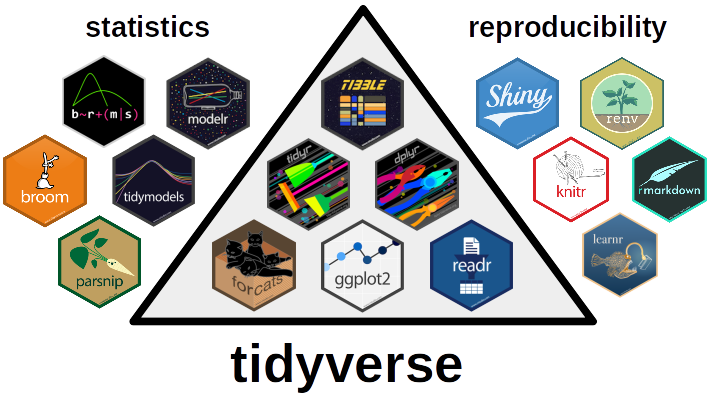
\includegraphics[width=0.8\linewidth]{tidyverse_ecosystem} 

}

\caption[Developing tidyqpcr using the tidyverse packages grants access to a larger ecosystem of data analysis packages.]{\textbf{Developing tidyqpcr using the tidyverse packages grants access to a larger ecosystem of data analysis packages.}}\label{fig:tidyverse-ecosystem}
\end{figure}

\textbf{Experimental design}  In tidyqpcr, we have built several plate plan helper functions built around block designs.
This enables samples to be spread across the plate and minimise well position biases but still contain regular patterns for loading with multi-channel pipettes, Figure \ref{fig:combined-plate-design}.
We also describe in detail different plate design strategies that users can explore depending on their pipettes and plates.
Users can exclude loading samples into edge wells with the provided helper functions.
We are also exploring introducing automatic generation of loading recipes for common liquid handlers so users with the access to the appropriate equipment can ensure the loader and plate plan match identically.
Therefore, grouping biological/technical replicates so they are place in the neighbouring wells could lead to systematic effects confounding biological effects.
This can compound even further if the same samples are place in the similar positions across multiple different wells. In an ideal situation, different samples and their replicates should be allocated entirely random well positions.
However, if the sample loading is manual, then having inconsistent loading plans across plates can lead to incorrect loading.
Ultimately, having an incorrect map of samples in wells is significantly more detrimental to any analysis than systematic bias.
A balance between easy loading and good experimental design principles are required.

\begin{figure}[p]

{\centering 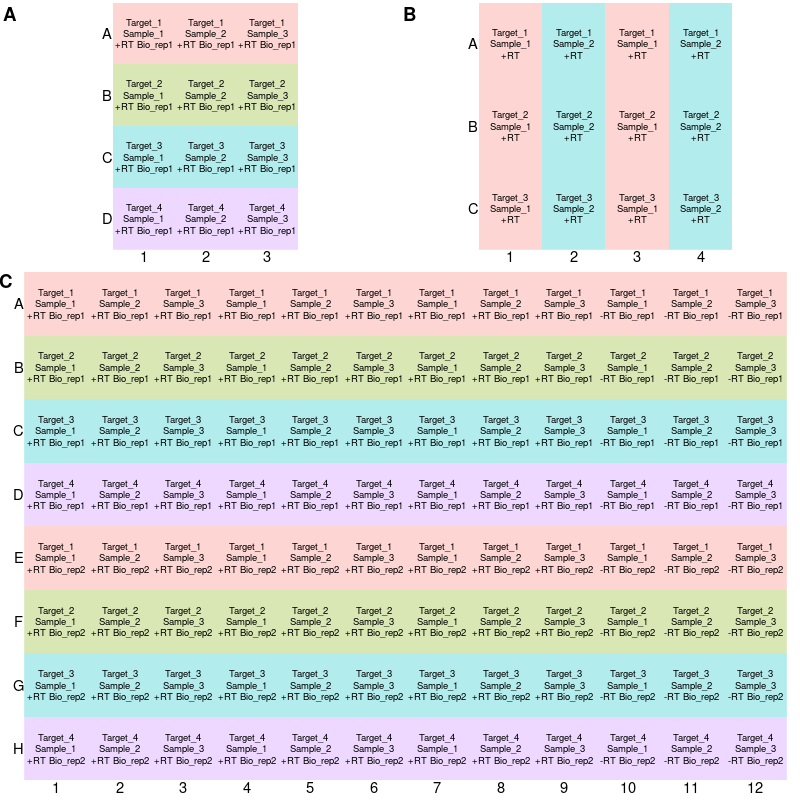
\includegraphics[width=1\linewidth]{combined_plate_plans.png} 

}

\caption[tidyqpcr facilitates flexible, modular plate design.]{\textbf{tidyqpcr facilitates flexible, modular plate design.} \textbf{(A)} Single repeatable block containing important well information: Sample\_id, target\_id, RT and bio\_rep number. 
\textbf{(B)} Alternative plate design with alternate sample replicates. Useful for pipetting with multi-channel pipettes. 
\textbf{(C)} Full 96 well plate design based on the repeatable block of panel \textbf{A}. 
Shows a MIQE-compliant plate with 3 technical replicates, 2 biological replicates and -RT controls.} \label{fig:combined-plate-design}
\end{figure}


\textbf{MIQE-compliant results} tidyqpcr follows the MIQE-guidelines for analysis by allowing multiple normalising genes by default in the delta-Cq calculation. 
Helper functions for the design of serial dilutions plates for primer calibration are available together with functions to calculate linearity, $R^2$ and plots to display behaviour across multiple primers.
Importing the fluorescence across all cycles is also available so that quality control graphs for the melt and amplification curves across all wells can be seen, Figure \ref{fig:plate-amp-curves}.
There are also default functions to plot Cq values across the plate to see biases, such as edge well bias. 
The vignettes also outline a reproducible analysis pipeline so users can ensure they complete all the necessary checks and to standardise analysis so reviewers can check analysis.
All vignettes also describe the use of technical replicates, biological replicates and control wells that contain RNA samples without reverse transcriptase.

\begin{figure}[t]

{\centering 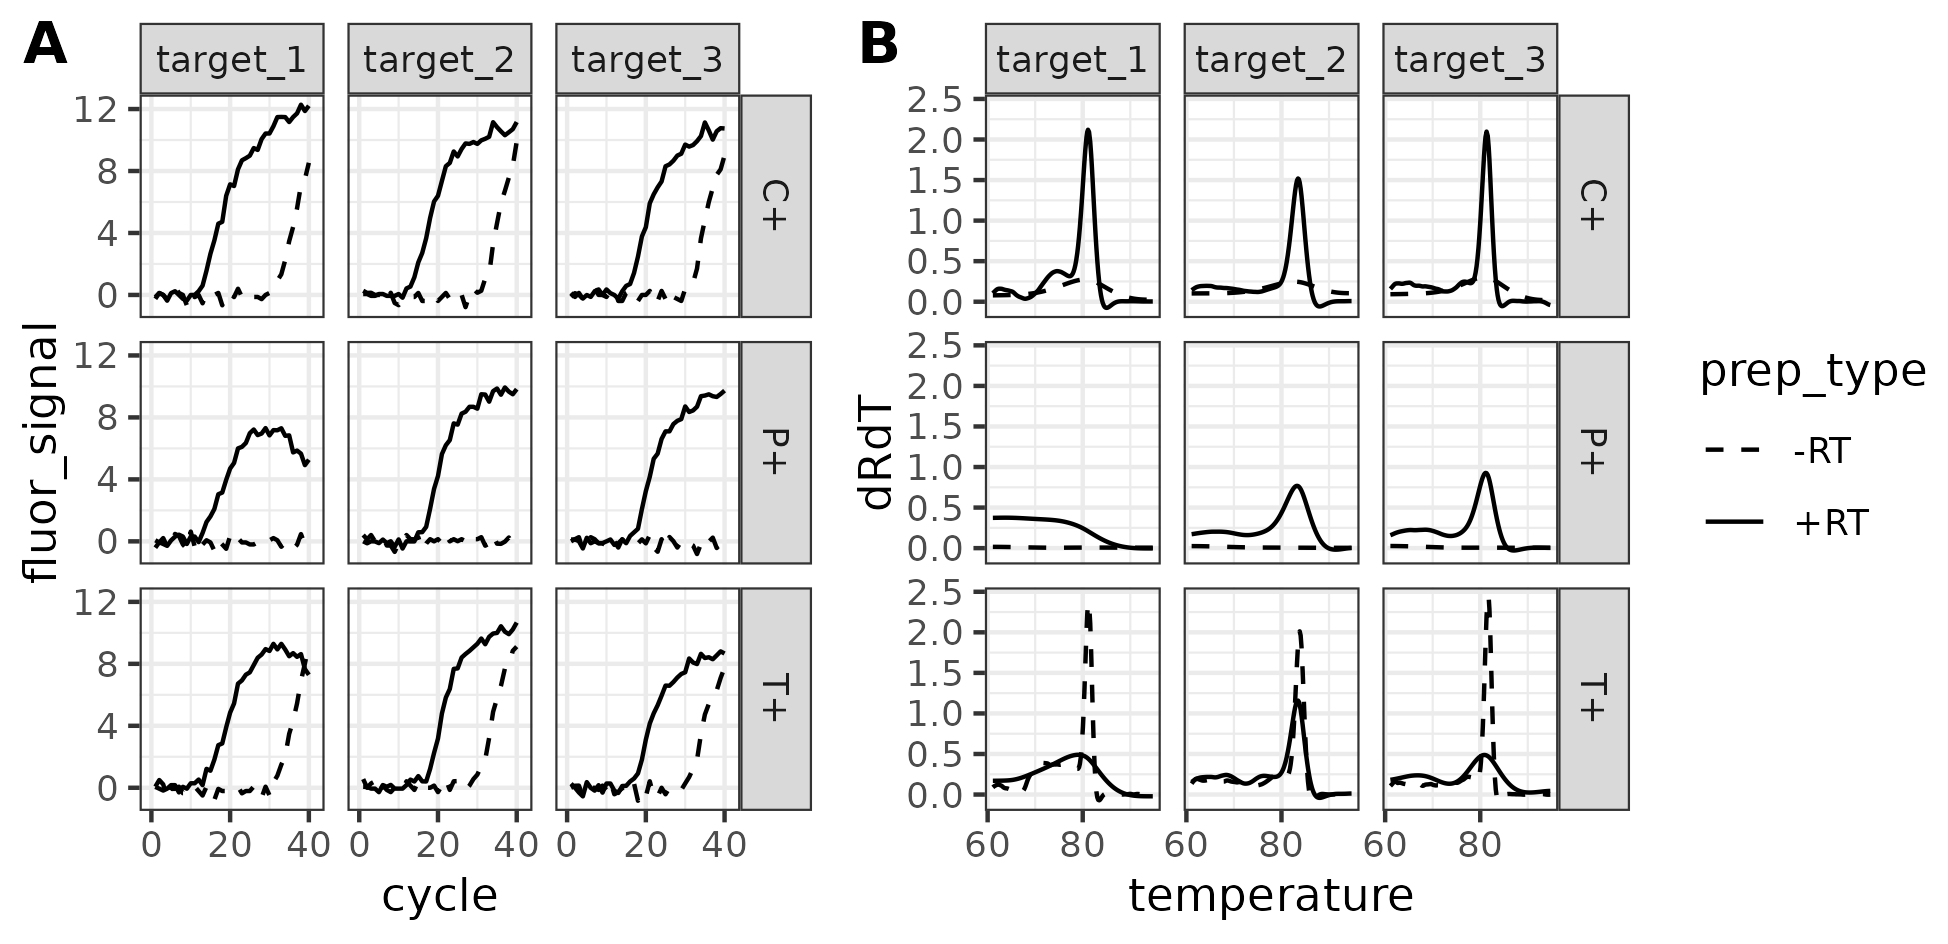
\includegraphics[width=1\linewidth]{example_melt_and_curve_plots.png} 

}

\caption[Extensive vignettes teach users MIQE-compliant analysis.]{\textbf{Extensive vignettes teach users MIQE-compliant analysis.} \textbf{(A)} Amplification curve plots verifying that curves of the control samples without reverse transcriptase (dotted lines) do not overlap with the samples of interest.
\textbf{(B)} Melt curves showing double stranded DNA fragments become single stranded above the threshold temperature for samples of interest.} \label{fig:plate-amp-curves}
\end{figure}

\subsubsection{Functionality}

\textbf{Overview}
tidyqpcr provides the functionality to aid with the implementation of qPCR assays from design to analysis. 
The design of complex plate plans is facilitated with the use of general plate formatting and labelling functions such as \lstinline{label_plate_rowcol} and \lstinline{create_blank_plate}. 
Meanwhile, helper functions that create commonly used 96 and 364 well plates are provided: \lstinline{create_colkey_4diln_2ctrl_in_24} and \lstinline{create_rowkey_4_in_16}. 
Once the plate has been designed, users can the import the completed qPCR assay data straight from the raw qPCR machine output. 
There are default functions for imported light cycler data \lstinline{read_lightcycler_1colour_raw} but users can create functions to import data from other machines as long as the end data frame is in a tidy format.
The import functions can be used to import threshold Cq values calculated from the qPCR  machine or the Cq values across cycles for the entire time course.
There are functions to conduct quality control on the imported data, as required by the MIQE guidelines. 
\lstinline{calculate_drdt_plate} calculates the derivative of the melt curve enabling the user to confirm amplification occurs only at one temperature.
Plate effects such as reducing efficiency at edge wells can be inspected using \lstinline{display_plate_value}.
Before the experiment of interest can be conducted, the amplification efficiency of the primers must be tested in order to ensure the assumptions of the qPCR threshold Cq comparisons are valid.
\lstinline{calculate_efficiency_bytargetid} enables users to calculate primer efficiency across targets given appropriate dilution assay data.
Finally, on the completion of the quality control steps user can calculate deltaCq and deltadeltaCq values from any combination of samples and target using \lstinline{calculate_deltacq_bysampleid} and \lstinline{calculate_deltadeltacq_bytargetid}. 
The mechanics around calculating deltacq across replicates and plates is enabled through the key words \lstinline{sample_id} and \lstinline{target_id}.
\lstinline{target_id} is intended to hold information about the target of the qPCR primers and \lstinline{sample_id} identifies the condition/strain/biorep information from each sample.
Both words are necessary in the plate data frame in order to use tidyqpcr functions. 
The decision to name them \lstinline{sample_id} and \lstinline{target_id} was a balance between being specific enough to avoid ambiguity, but general enough to enable a variety of qPCR assays to be incorporated.  

\textbf{Use Case}

\captionsetup[table]{list=no}

An example use case is now described to show the power of tidyqpcr to analyse a complex 96 well qPCR assay.
The data set is a real assay inspecting the change in expression of 16 gene associated with the yeast stress response.
Yeast samples are exposed to heat shock in the presence of transcriptional inhibitors.
The two transcriptional inhibitors are Phenanthroline and Thiolutin.
Therefore, there are six conditions: no inhibitor present with and without heat shock, Phenanthroline with and without heat shock, and Thiolutin with and without heat shock.
There are three technical replicates, two experimental replicates and each sample has a control which has not had any reverse transcriptase added.
The example code will design the plate for this experiment, read in the results of the Roche LightcyclerqPCR machine and calculate normalised Cq values for all target-condition combinations.

The first stage of conducting a qPCR experiment with tidyqpcr involves the designing a plate with the \lstinline{label_plate_rowcol} function, Table  \ref{create-plate-plan}. 
It requires three data frame arguments: a blank plate data frame holding the shape and number of wells to be used, a rowkey data frame holding row-wise experimental meta data and a colkey data frame holding column-wise experimental meta data.
The blank plate data frame can be any custom shape or size and follow any labelling system as long as each column and row is uniquely identifiable. 
tidyqpcr does provide boilerplate 96, 384 and 1024 well plates.
The tidyqpcr example vignettes encourage users to hold \lstinline{target_id} data in the rowkey data frame and \lstinline{sample_id} data in the colkey data frame.
These leads to entire rows containing the same primer and technical replicates and controls being grouped together, which helps reduce sample loading errors.
Typically, designing the rowkey is a simple task.
In this example there are the same number of rows as \lstinline{target_id}'s so the mapping is one to one.
In other cases, if the number of \lstinline{target_id}'s is a factor of the number of rows then the \lstinline{target_ids} are replicated until all rows are filled.
This pattern is an easy way of introducing biological replicates onto a plate. 
Designing the colkey can be more complicated as different combinations of conditions, replicates and controls need to be included.
Similar to the rowkey, if the number of unique samples is a factor of the number of columns then they can be repeated in blocks to represent the technical replicates and -rt control.
Although it is not strictly necessary to use \lstinline{label_plate_rowcol} to create a plate, we designed the function to encourage the users to design the plate in a logical row-wise and column-wise manner.
This leads to a intuitive and reproducible method to load the plate which minimises mistakes and increase efficiency. 

\begin{table}
\centering
\begin{tabular}{ |p{5.6cm}  p{5.6cm}|}
\hline
  \begin{lstlisting}[style=mystyle]
# list target_ids of primer sets
target_id_levels <- c("HOR7",
   "HSP12", "HSP26", "HSP78",
   "HSP104", "RTC3", "SSA4",
   "PGK1", "ALG9", "HHT2",
   "HTB2", "RPS3", "RPS13",
   "RPS15", "RPS30A", "RPL39")

# Set up experimental samples
heat_levels <- c("-", "+")
heat_values <- factor(
   rep(heat_levels, each = 3),
   levels = heat_levels)
drug_levels <- c("C", "P", "T")
drug_values <- factor(
   rep(drug_levels, times = 2),
   levels = drug_levels)
condition_levels <- paste0(
   drug_levels,
   rep(heat_levels, each = 3))
\end{lstlisting}
 & 
 \begin{lstlisting}[firstnumber=20,style=mystyle]
condition_values <- factor(
   condition_levels,
levels = condition_levels)
 
# create plate plan
rowkey <- tibble(
   well_row = LETTERS[1:16],
   target_id = factor(target_id_levels, 
    levels = target_id_levels))

colkey <- create_colkey_6_in_24(
   heat = heat_values,
   drug = drug_values,
   condition = condition_values)

plateplan <- label_plate_rowcol(
   create_blank_plate(
      well_row = LETTERS[1:16],
      well_col = 1:24),
   rowkey, colkey)
\end{lstlisting} \\ 
\hline
\end{tabular}
\caption*{Example tidyqpcr code for designing a 96 well qPCR plate for an assay with 16 target stress response genes across 6 conditions.}
\label{create-plate-plan}
\end{table}
After the qPCR experiment has been conducted, the next step is to read in the results, Table \ref{read-raw-data}. 
The function \lstinline{read_lightcycler_1colour_cq} is the default function in tidyqpcr for reading in the calculated threshold Cq values held in the excel file format used by Roche Lightcyclers. 
The complementary function \lstinline{read_lightcycler_1colour_raw} enables user to load the Cq values across the entire time course for plotting quality control figures. 
Users using qPCR machines other than a Roche Lightcycler currently need to create their own function for reading in Cq data. 
The plate plans defined above can then quickly match the Cq values with the sample meta data. It is vital that the row and column labelling used by the qPCR machine is repeated correctly in the plate design data frame. 
As can be seen in the example code, the scalability of tidyverse functions enables tidyqpcr to easy incorporate multiple experimental replicates without significant changes in the pipeline.
\begin{table}
\centering
\begin{tabular}{|p{5.6cm}  p{5.6cm}|}
\hline
 \begin{lstlisting}[firstnumber=40, style=mystyle]
 file_path_cq_plate1 <- 
    system.file("extdata",
      "Edward_qPCR_TxnInhibitors_
         HS_2018-06-15_
         plate1_Cq.txt.gz",
      package = "tidyqpcr")

plate1 <- file_path_cq_plate1 %>%
read_lightcycler_1colour_cq() %>%
   left_join(plateplan,
      by = "well") %>%
   mutate(biol_rep = "1",
      plate = "1")

file_path_cq_plate2 <-
   system.file("extdata",
   "Edward_qPCR_TxnInhibitors_
      HS_2018-06-15_
      plate2_Cq.txt.gz",
   package = "tidyqpcr")
\end{lstlisting} &
\begin{lstlisting}[firstnumber=60, style=mystyle]
plate2 <- file_path_cq_plate2 %>%
read_lightcycler_1colour_cq() %>%
  left_join(plateplan,
     by = "well") %>%
  mutate(biol_rep = "2",
     plate = "2")

# combine data from both plates into a single data frame
plates <- bind_rows(plate1,
   plate2) %>%
  unite(sample_id, condition,
     biol_rep, sep = "",
     remove = FALSE)
\end{lstlisting} \\
\hline
\end{tabular}
\caption*{Example tidyqpcr code for reading threshold Cq values from LightCycler qPCR machines and combining them with the designed plate plan.}
\label{read-raw-data}
\end{table}

Finally, to complete this example analysis the function \lstinline{calculate_deltacq_bysampleid} will normalise all the Cq values from the targets of interest to the normalising genes, Table \ref{calc-delta-cq}. 
Following the MIQE guidelines,  this function can accept multiple normalising \lstinline{target_ids} and calculate a mean or median value to subtract from all targets of interest. 
Again, using the flexibility of the tidyverse the mean Cq across any combination of samples, replicates and experiments can be calculated. 
This is possible because tidyqpcr consistently follows the tidy paradigm across all function outputs. 
The comparison of expression across all conditions and targets is plotted using ggplot2, Figure \ref{fig:tidyverse-ecosystem}.

\begin{table}
\centering
\begin{tabular}{| p{5.6cm}  p{5.6cm} |}
\hline
 \begin{lstlisting}[firstnumber=70, style=mystyle]
 platesnorm <- plates %>%
  filter(prep_type == "+RT") %>%
  calculate_deltacq_bysampleid(
     ref_target_ids = "PGK1")

platesmed <- platesnorm %>%
  group_by(sample_id, condition, biol_rep, heat, drug, target_id) %>%
  summarize(
    delta_cq = median(delta_cq,
       na.rm = TRUE),
    rel_abund = median(rel_abund,
       na.rm = TRUE))
 \end{lstlisting}& 
 \begin{lstlisting}[firstnumber=83, style=mystyle]
ggplot(data = platesmed) +
  geom_point(aes(x = target_id,
     y = rel_abund, 
     shape = biol_rep,
     colour = drug),
    position = position_jitter(
       width = 0.2,
       height = 0)) +
  facet_wrap(~heat, ncol = 3) +
  scale_y_log10("mRNA relative detection",
     labels = scales::label_number()) +
  theme(axis.text.x = 
     element_text(angle = 90,
        vjust = 0.5))
\end{lstlisting}   \\
\hline
\end{tabular}
\caption*{Example tidyqpcr code for for calculating $\Delta$Cq across multiple plates and plotting summary results across target genes.}
\label{calc-delta-cq}
\end{table}

\begin{figure}[t]

{\centering 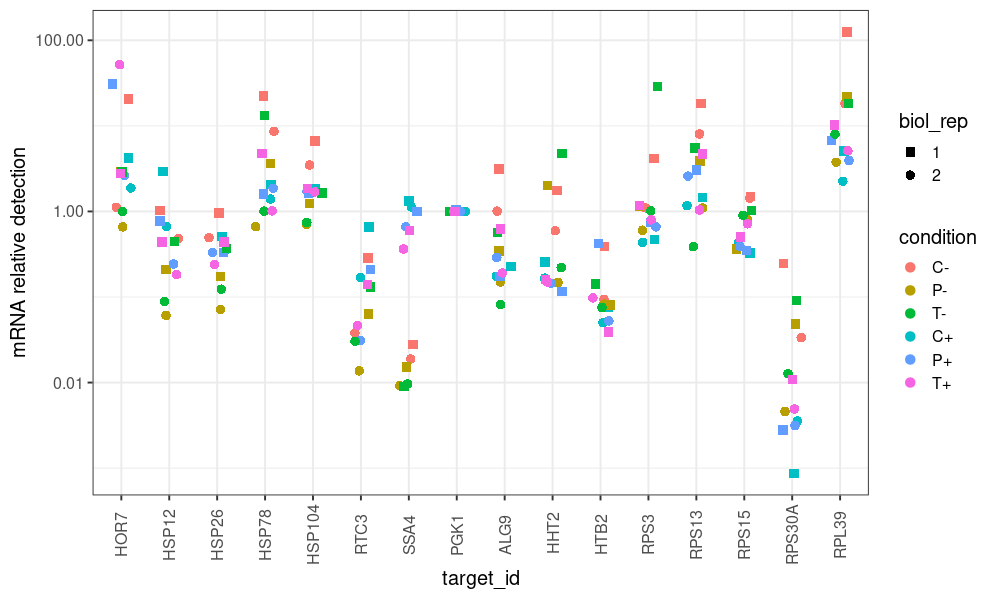
\includegraphics[width=\linewidth]{example_normalised_deltacq_multiplate_figure}}

\caption[tidyqpcr can be used to quickly analyse multi-plate, multi-target, and multi-sample qPCR assays.]{\textbf{tidyqpcr can be used to quickly analyse multi-plate, multi-target, and multi-sample qPCR assays. }}\label{fig:tidyqpcr-multi-plate}
\end{figure}

\textbf{Function definitions and Documentation}

tidyqpcr functions are designed following the tidyverse guidelines for compatible functions, Table \ref{define-function}. 
The verb-object nomenclature is followed throughout to help ensure each function is clearly named according to its purpose. 
The first argument of any tidyqpcr function is the primary data frame to be acted on. 
This allows the pipe operators commonly used in tidyverse code to continue their primary function. 
The input data frame is expected to be in the long tidy format and the outputs of any tidyqpcr function is also a data frame in long tidy format. 
The definition of the \lstinline{calculate_deltacq_bysampleid} function has been copied below as an example of a typical function code. 
The function groups cq values by \lstinline{sample_id} and subtracts the normalising \lstinline{target_id} values from all cq value in each group. 
Therefore, cq, \lstinline{sample_id}, and \lstinline{target_id} are vital variables and are checked to be in the supplied data frame before the function attempts to calculate deltacq. 
Once the presence of the required variables is asserted, the function calculates deltacq and adds it as a new variable to the data frame. 
The function is entire scalable as the internal \lstinline{group_by} function can handle any number of \lstinline{sample_id} and the deltacq's can be calculated by any number of normalising \lstinline{target_ids}.



\begin{table}
\centering
\begin{tabular}{| p{5.6cm}  p{6.1cm} |}
\hline
\begin{lstlisting}[style=mystyle]
calculate_deltacq_bysampleid <- 
 function(cq_df,
          ref_target_ids,
          norm_function = median) 
{

 assertthat::assert_that(
  assertthat::has_name(
   cq_df, 
   c("target_id",
     "sample_id",
     "cq")))
     
 cq_df %>%
  dplyr::group_by(
   .data$sample_id) %>%
\end{lstlisting} &

\begin{lstlisting}[firstnumber=17, style=mystyle]
   dplyr::do(
    calculate_normvalue(
     .data,
     ref_ids = ref_target_ids,
     value_name = "cq",
     id_name = "target_id",
     norm_function = 
      norm_function)) %>%
  dplyr::rename(
   ref_cq = 
    .data$value_to_norm_by) %>%
      dplyr::ungroup() %>%
      dplyr::mutate(
       delta_cq = 
        .data$cq - .data$ref_cq,
       rel_abund = 
        2^ -.data$delta_cq)}
\end{lstlisting} \\
\hline
\end{tabular}
\caption*{Function definition for the calculate $\Delta$Cq method within tidyqpcr.}
\label{define-function}
\end{table}
Preceding the function definition is several commented lines documenting the details and use cases of the function, Table \ref{function-documentation}. 
First, a brief description of the function, its input arguments and expected output is provided. 
Then, its dependencies on other functions both inside tidyqpcr and in other R packages are listed. 
Finally, short examples showing the use of the function are outlined. 
This preamble is converted into markdown formatted help documentation by the r package roxygen2. 
This documentation is accessible using the base help command once tidyqpcr has been downloaded and as a standalone documentation website hosted by ropensci.
\begin{table}
\centering
\begin{tabular}{| p{6.1cm}  p{5.6cm} |}
\hline
\begin{lstlisting}[style=mystyle]
#' Calculate delta cq to normalize 
#, quantification cycle (log2-fold)
#' data within sample_id.
#'
#' This function implements 
#' relative quantification by the 
#' delta Cq method. For each 
#' sample, the Cq values of all 
#' targets (e.g. genes, probes, 
#' primer sets) are compared to 
#' one or more reference target 
#' ids specified in 
#' `ref_target_ids`.
#'
#' @param cq_df a data frame 
#'  containing columns `sample_id`,
#'  value_name (default `cq`) and
#'  tid_name (default `target_id`).
#'  Crucially, sample_id should be
#'  the same for different technical
#'  replicates measuring identical 
#'  reactions in different wells of 
#'  the plate, but differ for 
#'  different biological and 
#'  experimental replicates. See 
#'  tidyqpcr vignettes for examples.
#' @param ref_target_ids names of 
#'  targets to normalize by, i.e. 
#'  reference genes, hydrolysis 
#'  probes, or primer sets. This can 
#'  be one reference target id,
#'  a selection of multiple target
#'  ids, or even all measured 
#'  target ids. In the case of all 
#'  of them, the delta Cq value 
#'  would be calculated relative to
#'   the median (or other 
#'  `norm_function`) of all measured 
#'  targets.
#' @param norm_function Function to 
#'  use to calculate the value to
#'  normalize by on given scale. 
#'  Default is median, alternatively 
#'  could use mean.
#'
#' @return data frame like cq_df 
#'  with three additional columns:
#'   ref_cq,  cq value for reference 
#'            target ids;
#'   delta_cq,  normalized value;
#'   rel_abund, normalized ratio.
\end{lstlisting} &
\begin{lstlisting}[firstnumber=52, style=mystyle]
#' @export
#' @importFrom tidyr %>%
#' @importFrom stats median
#' @importFrom rlang .data
#' @examples
#' # create simple cq dataset 
#' # with two samples, two 
#' # targets  and 3 reps
#'
#' cq_tibble <- tibble(
#'  sample_id = rep(
#'   c("S_1", "S_1", "S_1", 
#'     "S_2", "S_2", "S_2"),
#'     2),
#'  target_id = rep(
#'   c("T_1",
#'     "T_norm"),
#'   each = 6),
#'  tech_rep = rep(1:3, 4),
#'  well_row = rep(
#'   c("A", "B"),
#'   each = 6),
#'  well_col = rep(1:6, 2),
#'  well = paste0(well_row,
#'                well_col),
#'  cq = c(10, 10, 10, 12,
#'         12, 11,  9,  9, 
#'          9,  9,  9,  9))
#'                      
#' # calculate deltacq using
#' # reference target_id 
#' # called 'T_norm'
#' 
#' # use case 1: 
#' # median reference 
#' # target_id value
#'
#' cq_tibble %>%
#'  calculate_deltacq
#'       _bysampleid(
#'    ref_target_ids = "T_norm")
#' 
#' # use case 2: 
#' # mean reference target_id 
#' # value 
#'
#' cq_tibble %>%
#'  calculate_deltacq
#'           _bysampleid(
#'   ref_target_ids = "T_norm",
#'   norm_function = mean)
\end{lstlisting} \\
\hline
\end{tabular}
\caption*{Function documentation for the calculate $\Delta$Cq method within tidyqpcr as dictated by the roxygen2 R package.}
\label{function-documentation}
\end{table}
\newpage
\textbf{Tests}

tidyqpcr follows software development best practices by incorporating unit tests for all vital functions within the package, Table \ref{function-tests}. 
95\% of all functions within tidyqpcr are covered by a test. 
The development on tidyqpcr uses the continuous integration available in GitHub as a GitHub Action runs each unit test to check for bugs with every commit to the repository. 
The tests consist of small use cases with the simplest expected outcome from each function is created and compared to the actual output. 
Functions with multiple possible behaviours according to optional arguments have multiple tests ensure function logic performs as expected. 

\begin{table}
\centering
\begin{tabular}{| m{10cm} |}
\hline
\begin{lstlisting}[style=mystyle]
test_that("Unit test for the calculate_deltacq function",
{
   simulated_48_well_plate_plan <- create_blank_plate_96well() %>%
      dplyr::filter(well_row %in% c("A", "B",
                                    "C", "D")) %>%
      dplyr::mutate(
         target_id = rep(c("Target_1", "Target_2",
                           "Target_3", "Target_4"),
                         each = 12),
         sample_id = rep(rep(c("Sample_1", "Sample_2",
                               "Sample_3"),
                             each = 4),
                         times = 4),
         tech_rep = rep(c(1, 2, 3, 1),
                        times = 12),
         prep_type = rep(c("+RT", "+RT",
                           "+RT", "-RT"),
                         times = 12))

   calculated_48_well_plate_with_deltacq <- 
      calculate_deltacq_bysampleid(
         simulated_48_well_plate_with_cq %>%
            dplyr::filter(prep_type == "+RT"), 
         ref_target_ids = "Target_3") %>%
            dplyr::arrange(well_row, well_col)

    expect_equal(calculated_48_well_plate_with_deltacq,        
                 simulated_48_well_plate_with_deltacq)})
\end{lstlisting} \\
\hline
\end{tabular}
\caption*{Function test for the calculate $\Delta$Cq method within tidyqpcr as dictated by the testthat R package.}
\label{function-tests}
\end{table}

\captionsetup[table]{list=yes}
\setcounter{table}{0}

\subsection{Reviewing and improving tidyqpcr}

\subsubsection{Themes derived from semi-structured interviews}

We conducted a series of semi-structured interviews to explore current practices in qPCR experimental design and analysis.
These interviews where conducted over zoom with the video recorded by zoom's proprietary software over a period between 45 and 90 minutes.
The interview explored whether users were aware of the MIQE guidelines and if they currently executed any QC measures. 
We also wanted to know about the typical experiments users conducted; i.e. qPCR machine, reagents, and plate plans. 
Finally, we wanted to explore what software users currently used to analyse their results and if they were interested in learning R based analysis. 
The questions guiding the interview are available in Appendix B.
The six interviewees covered several academic roles from senior post-doctoral research assistants to undergraduates.
The interviewees had varied experiences in programming based analysis and in conducting qPCR assays.
The transcripts from the interviews are available in Appendix C.
Once the interview was completed the interviewers were introduced to tidyqpcr and asked to complete a user test.

Several key themes relating to the design and analysis of qPCR experiments appeared across the interviews, Figure \ref{fig:semi-structured-test-cloud}.
In terms of the design of qPCR assays all interviewees reported doing RNA not DNA quantification.
The inclusion of three technical replicates was typical although some users had a process of removing outliers.
It also was not common practice to check amplification curves or confirm linear efficiency.
Overall, few were aware of the MIQE guidelines and few recall published data giving QC results, analysis code or detailed protocols.
In addition, no-one reported trying to recreate any other published data set and a regular theme of not trusting conclusions based on qPCR results alone was common.
In terms of the analysis of qPCR data Rxcel remains a common piece of software for the analysis and design of plates.
Users almost universally depend on qPCR machine software to determine Cq values.
Few were aware of the concept of 'tidy' data outside of users already using R packages  based on the tidyverse.
Although most users are confident they could re-analysis their own results no-one reported that their analysis was openly available for reviewers to access.

\begin{figure}[t]

{\centering 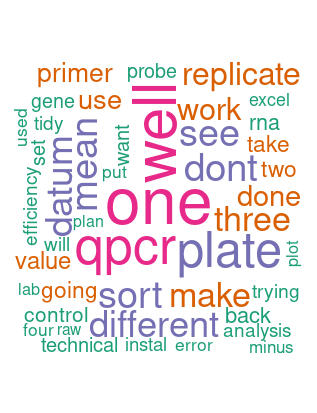
\includegraphics[width=0.5\linewidth]{mg_rb_ck_ec_db_semi_structured_word_cloud} 

}

\caption[A text cloud showing the key words repeatedly used across the semi-structured interviews.]{\textbf{A text cloud showing the key words repeatedly used across the semi-structured interviews.} The greater the frequency of a word the larger it appears in the figure. }\label{fig:semi-structured-test-cloud}
\end{figure}

\subsubsection{rOpenSci review and JOSS submission}
In order to ensure tidyqpcr followed best software development practices and to verify the reliability of its functions, we submitted the package for an rOpenSci code review. 
rOpenSci offers transparent, constructive and open reviews of R packages that lower barriers to working with local and remote scientific data sources.
A successful rOpenSci review can then be submitted to the Journal of Open Source Software (JOSS), enabling the software development work to be officially acknowledged with a citation.
The submission to JOSS was publish in June 2022, \url{https://joss.theoj.org/papers/10.21105/joss.04507}.

The rOpenSci review highlighted several issues with tidyqpcr's implementation, including: insufficient compliance with FAIR software practices, failing CRAN software repository checks, and the inclusion of redundant functionality. 
rOpenSci requires all submitted software to be Findable, Accessible, Interoperable and Reusable (FAIR) and follow the practices of the CodeMeta Project (\url{https://codemeta.github.io/}).
rOpenSci required us to add an codemeta.json file which standardises how the meta data associated with the software is held, such as maintainer details or software dependencies.
Standardising the format of the meta data ensures a) all the data required to reuse a piece of software is available, and b) search functions can be developed to find software based on different meta data tags.
Acceptance in to rOpenSci suite of peer reviewed packages also includes submission to the R package repository CRAN.
However, the example data sets and extensive vignettes included in the tidyqpcr package led to it being over 5Mb, which is too large to be hosted on CRAN.
We managed to reduce the package size by converting the example data set files to compress zip files.
It was also highlighted that some functions originally packaged within tidyqpcr to aid with producing interpretable graph labels appeared out of place.
We removed these plot helper functions as the scales package also provided the functionality \parencite{Wickham2022}.

\subsubsection{User Feedback}
Following the Agile software development practice, feedback from users was used to influence development priorities at regular intervals. 
Feedback was acquired from multiple sources: user testing following the user interviews outlined above, an independent code by a bioinformatics research assistant and from the rOpenSci code review.
The task-based  user test section of the interview focused on three main themes of tidyqpcr: block based plate planning, tidyverse based API and conducting reproducible analysis.
Meanwhile, an independent code review following the Google code review guidelines was conducted by a colleague who had not previously contributed to the development of tidyqpcr.
An overview of major improvements to tidyqpcr's functionality, usability, and documentation in response to user feedback is available in Table \ref{user-feedback}.

\begin{table}
\centering
\begin{tabular}{|| m{4.5cm} | m{7cm} ||} 
 \hline
 \textbf{\large Issue} & \textbf{\large Solution} \\ [0.5ex] 
 \hline\hline
 \multicolumn{2}{|l|}{\textbf{Functionality}} \\
 \hline
 tidyqpcr contains helper functions to create 96 and 384 well plates but 1536 plate wells are not supported. & 
 Created a helper function to automatically create 1536 plate as well as a function to produce a "pick list" based on the plate to facilitate the use of robotic sample loaders (echo liquid handler). \\ 
 \hline
 Quality control should include a method for checking for positional effects on a qPCR plate. & 
 Created the display\_plate\_value function to visualise threshold Cq values across the plate following the user defined plate plan. \\
 \hline
 \multicolumn{2}{|l|}{\textbf{Usability}} \\
 \hline
 Determining general but intuitive names for function arguments. & 
 Depending on assay used the measurement variable could be called Primer Set (for SYBR dye-style) or a fluorescent-quenched probe (Taqman). 
 Rather than committing to a specific assay we decided on the more general term target\_id. \\
 \hline
 The benefit of using tidyqpcr over the other available packages remains unclear. & 
 The GitHub Repo README file now contains a summary table comparing functionality and MIQE compliance across tidyqpcr and its popular alternative packages.\\
 \hline
 \multicolumn{2}{|l|}{\textbf{Documentation}} \\
 \hline
 Current package vignettes overwhelm new users as they introduce the basic concepts of tidyqpcr on multi-condition, multi-target data sets. & 
 Interviewee provided a simpler 96-well plate data set for us to use as an example. 
 We created a simpler vignette introducing the basic concepts of tidyqpcr using this data set for users to understand before moving onto the larger example. \\
 \hline
\end{tabular}
\caption[tidyqpcr development cycle included regular improvements from user feedback.]{tidyqpcr development cycle included regular improvements from user feedback.}
\label{user-feedback}
\end{table}

\subsubsection{Future functionality}

tidyqpcr is a fully self-sufficient package for the analysis of qPCR data using SYBR Green assays from Roche Lightcycler qPCR machines. 
However, there remains several planned improvements to enable tidyqpcr to easily analyse data from other qPCR assays and major additions to complete its aim to analyse qPCR data in an entirely open way according to the MIQE guidelines.
First, to extend the import functions to read formats from other qPCR machines we intend to incorporate the plater R package \parencite{Hughes2016}.
This package follows the same tidy data principles as tidyqpcr, but is built to read data formats from a variety of qPCR machines.
Next, tidyqpcr has only been tested to work on SYBR Green qPCR assays.
Taqman based qPCR assays allow multiplexing so each well can measure multiple targets. 
Acquiring suitable Taqman data and add documentation on how tidyqpcr can be used to analysis such assays would also lead to addition functionality. 

The previous improvements enhance the use cases of tidyqpcr, but tidyqpcr needs additional functionality to complete its MIQE compliant and open source aims.
The major additions are: to include primer efficiency into delta Cq calculations, to provide methods to determine appropriate normalising genes, to import and export qPCR meta data in RDML form, and to calculate threshold Cq values itself. 
geNorm is an established method for incorporating primer efficiency into Cq values 
Meanwhile, the R package NormqPCR already contains the functionality to determine appropriate normalising genes to determine deltaCq values from a group of candidate genes. 
Integrating the geNorm method and NormqPCR functionality within the \lstinline{calculate_normvalue} is a priority.
As the default file type for MIQE compliant qPCR analysis, creating the functionality to update RDML files using the RDML R package would increase the ease of conducing MIQE compliant qPCR assays \parencite{Roediger2017}.
Finally, tidyqpcr needs to remove its reliance on the threshold Cq value calculations conducted by proprietary software in qPCR machines. 
There are multiple methods to determine threshold Cq values the majority are available within the qpcR R package described above.
Integrating the comprehensive set of functions in qpcR in a tidy format usable by tidyqpcr should complete the open source requirement from tidyqpcr's statement of intent. 

\section{Chapter 3 Conclusion}

qPCR remain one of the most widely used microbiology assays with uses across medicine, law and biology. However, awareness of what is required for someone else to repeat an experiment remains a key obstacle in ensuring reliable, reproducible results. 
Solutions have been widely published, such as the MIQE guidelines, but few publications appear to follow them. 
In addition, surveying the current qPCR analysis software landscape it is clear that there remains a gap in accessible, reproducible and scalable analysis packages. 
Therefore, a combination of low levels of awareness and high levels of required effort impedes the publication of protocols and analyses in an open way. 
The consequences of the lack of reproducibility continues to have a detrimental effect on the quality and reliability of conclusions based on qPCR data. 
In summary, there remains a serious demand for methods that support and teach the best practices in qPCR assay design and analysis.


Here, we have described the R package tidyqpcr which aims to facilitate the analysis of qPCR data in an open, reproducible and reliable way. 
Created using best practices in open source software development, the expansive tidyverse suite of data analysis packages and the MIQE guidelines we believe this tool can help experimentalists improve the quality of their analysis and the confidence in their results.
We utilised the full suite of documentation pathways available in R to enable users to access the required level of detail for their expertise. 
Step-by-step workflows are provided in detail in the vignettes with specific reference to the MIQE guidelines and experimental plans that include controls, replicates, and block designs. 
More experienced programmers can take advantage of the complete function documentation to cherry pick the steps they required and combine with the plethora of tidyverse packages to create bespoke pipelines of their own.
We believe that the extensive work put in to ensure the package is an open and accessible as possible will manifest in to users contributing their own improvements and functions to the package. 
The initial response from users outside of our lab have been overwhelming positive suggesting this package can improve the quality and clarity of results across the wider research community.
\end{document}